%%%%%%%%%%%%%%%%%%%%%%%%%%%%%%%%%%%%%%%%%
% University/School Laboratory Report
% LaTeX Template
% Version 3.1 (25/3/14)
%
% This template has been downloaded from:
% http://www.LaTeXTemplates.com
%
% Original author:
% Linux and Unix Users Group at Virginia Tech Wiki 
% (https://vtluug.org/wiki/Example_LaTeX_chem_lab_report)
%
% License:
% CC BY-NC-SA 3.0 (http://creativecommons.org/licenses/by-nc-sa/3.0/)
%
%%%%%%%%%%%%%%%%%%%%%%%%%%%%%%%%%%%%%%%%%

%----------------------------------------------------------------------------------------
%	PACKAGES AND DOCUMENT CONFIGURATIONS
%----------------------------------------------------------------------------------------

\documentclass{article}

%\usepackage[version=3]{mhchem} % Package for chemical equation typesetting
\usepackage{graphicx} % Required for the inclusion of images
\usepackage{natbib} % Required to change bibliography style to APA
\usepackage{amsmath} % Required for some math elements 
\usepackage[utf8]{inputenc} % Required for special characters processing
\usepackage{url}
%
\usepackage{fullpage} % changes the margin
\usepackage{siunitx} % Provides the \SI{}{} and \si{} command for typesetting SI units
\newcommand{\gc}{\degreeCelsius}
\usepackage{pdflscape} % Change text sections orientation
%
\setlength\parindent{0pt} % Removes all indentation from paragraphs

\renewcommand{\labelenumi}{\alph{enumi}.} % Make numbering in the enumerate environment by letter rather than number (e.g. section 6)

\usepackage{times} % Uncomment to use the Times New Roman font

%----------------------------------------------------------------------------------------
%	DOCUMENT INFORMATION
%----------------------------------------------------------------------------------------

\title{\textbf{Meteorology Report Codes} \\ Meteorology
  \& Climatology} % Title

\author{Environmental Science Degree} % Author name

\date{\today} % Date for the report

\begin{document}

\maketitle % Insert the title, author and date

\begin{center}
\begin{tabular}{l r}
Date Performed: & \underline{\hspace{3cm}}  \\ % Date the experiment was performed
Partners: & \underline{\hspace{6cm}} \\ % Partner names
& \underline{\hspace{6cm}} \\
& \underline{\hspace{6cm}} \\
Instructor: & Prof.~F.~Pérez-Bernal % Instructor/supervisor
\end{tabular}
\end{center}

% If you wish to include an abstract, uncomment the lines below
\begin{abstract}
This lab session aim is to present meteorology report codes, in
particular the SYNOP code. Students should
learn to encode a general weather situation to this code as well as to
interpret the code both graphically and as a short weather report.
\end{abstract}

%----------------------------------------------------------------------------------------
%	SECTION 1
%----------------------------------------------------------------------------------------
\section{Introduction}
% is a format for reporting weather information. A METAR weather
% report is predominantly used by pilots in fulfillment of a part of a
% pre-flight weather briefing, and by meteorologists, who use
% aggregated METAR information to assist in weather forecasting.

SYNOP stands for \textit{surface SYNOPtic observation} and it is a numerical
code (called FM-12 by the World Meteorological Office WMO\cite{FM-12}) that has been used for decades as the main way of reporting and transmitting
weather information. The observations could be made by manned and automated weather stations. 

The international SYNOP format has been used for real time transmission of synoptic weather observations for about 50 years and SYNOP reports are typically sent every six hours by Deutscher
Wetterdienst on shortwave and low frequency using RTTY. The
introduction of Internet made this redundant.

A report consists  of groups of five numbers (and slashes
where data are not  available) describing general weather information,
such  as  the temperature,  atmospheric  pressure, precipitation,  and
visibility at a weather station.

In most countries, SYNOP observations are made and transmitted each 3
hours at 0000, 0300, 0600, 0900, 1200, 1500, 1800, and 2100 Universal
Time (UTC). There are two basic forms of land station surface synoptic
reports, one of which is the complete form and the other is the
shortened form. The complete form is referred to as the primary (or
main) synoptic, the 6-hourly report, or SYNOP. The primary synoptic is
reported at the standard hours of observation which are: 0000, 0600,
1200, and 1800 UTC. The shortened form is referred to as the
intermediate synoptic or the 3-hourly report.

The SYNOP code is very similar to a different code, the METAR. METAR
is an abbreviation of \textit{MÉTéorologique Aviation Régulière} and
is a report designed for aviation that could be issued from an
Automatic Weather Station (AWS) or a manned station. The METAR code is
also managed by the WMO. METARs usually carry less information aboutr
the weather than SYNOPs and are issued more frequently. In particualr,
if conditions change significantly since the last METAR, a SPECI, or
specia weather report is produced. SPECIs are sent to report heavy
rain, sudden increase or direction change of wind, strong gusts, or
sudden temperature or visibility variations.

\section{Objectives}
Theo objective of this lab session is that student get acquainted with SYNOP code and make them able to codify a given weather report as well as decodify it and prepare a graphical representation.


\section{Synop Code Description and Lab Procedures}

The general syntax of the SYNOP code is as follows
\begin{align*}
&IIiii \text{ or } IIIII\; YYGGi_w\; 99LLL\; QLLLL\\
&i_Ri_XhVV\; Nddff\; 00fff\; 1sTTT\; 2sTTT\; 3PPPP\; 4PPPP\; 5appp\; 6RRRt\; 7wwW_1W_2\; 8NC_LC_MC_H\; 9GGgg\\
&222Dv\; 0sTTT\; 1PPHH\; 2PPHH\; 3dddd\; 4PPHH\; 5PPHH\; 6IEER\; 70HHH\; 8aTTT\\
&333\; 0....\; 1sTTT\; 2sTTT\; 3Ejjj\; 4Esss\; 5jjjj\; jjjjj\; 6RRRt\; 7RRRR\; 8Nchh\; 9SSss
\end{align*}

Very few reports will use all of the groups. For example, only at a coastal station would the section 222 (wave
information) be included, and even that station might not include all of the groups in the 222
section. Also, individual groups may be left out of an observation for a number of reasons.
Different regions may have requirements which will include groups or exclude groups,
principally in section 333.


There are four main groups:

\begin{description}
\item{000 Group} Identification and Location
\item{111 Group} Land Observations
\item{222 Group} Sea Surface Observations
\item{333 Group} Climatological Data
\end{description}

\subsection{000 Group: Identification and Location}

\begin{description}
\item[$IIiii$] The WMO number of the station\cite{ogimet}.
\item[$IIIII$] Ship or Buoy Observations.The ship or buoy identifier.
\item[$YYGGi_w$]
  \begin{tabular}{cl}
    $YY$ & The day of the month\\
    $GG$ & The hour of the observation (UTC)\\
    $i_w$ & Wind type indicator\\
    0  & m/s (estimated)\\
    1  & m/s (from anemometer)\\
    2  & knots (estimated)\\
    3  & knots (from anemometer)
  \end{tabular}
\item[$99LLL QLLLL$]
  \begin{tabular}{cl}
    $LLL$ & Latitude of observation to .1 degrees\\
    $Q$ & Quadrant of observation\\
    1 & North east \\
    3 & South east\\
    5 & South west\\
    7 & North west\\
    $LLLL$ & Longitude of  observation to .1 degrees
  \end{tabular}
\end{description}

\subsection{111 Group: Land Observations}

\begin{description}
\item[$i_Ri_XhVV$]
  \begin{description}
  \item[$i_R$] -- Precipitation indicator
    \begin{tabular}{cl}
      0 & Precipitation in groups 1 and 3\\
      1 & Precipitation reported in group 1 only\\
      2 & Precipitation reported in group 3 only\\
      3 & Precipitation omitted, no precipitation\\
      4 & Precipitation omitted, no observation
    \end{tabular}
  \item[$i_X$] -- Station type and present/past weather indicator
    \begin{tabular}{cll}
      Value & Station & Weather group\\
      1 & manned  &included\\
      2 & manned  &omitted, no significant weather\\
      3 & manned  &omitted, no weather observation\\
      4 & automated  & included (see automated codes 4677 and 4561)\\
      5 & automated  & omitted, no significant weather\\
      6 & automated  & omitted, no weather observation\\
      7 & automated  & included (see automated codes 4680 and 4531)\\
    \end{tabular}
  \item[$h$] -- Cloud base of lowest cloud seen (meters above ground)
    \begin{tabular}{cl}
      0 & 0 to 50 m \\
      1 & 50 to 100 m \\
      2 & 100 to 200 m\\
      3 & 200 to 300 m\\
      4 & 300 to 600 m\\
      5 & 600 to 1000 m\\
      6 & 1000 to 1500 m\\
      7 & 1500 to 2000 m\\
      8 & 2000 to 2500 m\\
      9 & above 2500 m\\
      / & unknown\\
    \end{tabular}
  \item[$VV$] -- Visibility
    \begin{tabular}{lllll}
      00 $<$ 0.1 km & 01 -- 0.1 km & 02 -- 0.2 km & ... & 50 -- 5.0 km\\
      56 -- 6 km          & 57 -- 7 km   & 58 -- 8 km   & ... & 80 -- 30 km \\
      81 -- 35 km         & 82 -- 40 km  & 83 -- 45 km  & 84 -- 50 km & 85 -- 55 km\\
      86 -- 60 km         & 87 -- 65 km  & 88 -- 70 km  & 89 -- $>$ 70 km & \\
      90 -- $<$ 0.05 km     &91 -- 0.05 km & 92 -- 0.2 km & 93 -- 0.5 km & 94 -- 1 km\\
      95 -- 2 km          &96 -- 4 km    & 97 -- 10 km & 98 -- 20 km & 99 -- $>$ 50 km\\
      // -- missing       &              &             &             &               \\
    \end{tabular}
  \end{description}
\end{description}
\begin{description}
\item[$Nddff$]
  \begin{description}
  \item[$ N$] -- Total cloud cover
    \begin{tabular}{llllll}
      0 -- clear & 1 -- 1/8th & 2 -- 2/8ths & 3 -- 3/8ths &  4 -- 4/8ths& 5 -- 5/8ths \\
      6 -- 6/8ths& 7 -- 7/8ths & 8 -- overcast & 9 -- sky obscured & &/ -- no observation
    \end{tabular}
  \end{description}
\item[$dd$] -- wind direction in 10s of degrees 
\item[$ff$] -- wind speed in units determined by wind type indicator (see above)
\end{description}
\begin{description}
\item[$00fff$ (optional)]
  \begin{description}
  \item[$fff$] -- wind speed if value greater than 100
  \end{description}
\end{description}
\begin{description}
\item[$1sTTT$] -- Temperature
  \begin{description}
  \item[$s$] -- sign of temperature (0=positive, 1=negative)
  \item[$TTT$] -- Temperature in \SI{0.1}{\gc}
  \end{description}
\end{description}
\begin{description}
\item[$2sTTT$] -- Dewpoint
    \begin{description}
    \item[$s$] -- sign of temperature (0=positive, 1=negative, 9 = RH)
    \item[$TTT$] -- Dewpoint temperature in \SI{0.1}{\gc} (if $s$ is 9, $TTT$ is relative humidity)
  \end{description}
\end{description}
\begin{description}
\item[$3PPPP$] -- Station pressure in \SI{0.1}{hPa} (thousandths digit omitted, last digit can be slash, then pressure in full \si{hPa})
\end{description}
\begin{description}
\item[$4PPPP$] -- Sea level pressure in \SI{0.1}{hPa} (thousandths digit omitted, last digit can be slash, then pressure in full \si{hPa})
\end{description}
\begin{description}
\item[$4a_3hhh$] -- Geopotential of nearest mandatory pressure level (use for high altitude stations where sea level pressure reduction is not accurate)
  
  \begin{description}
  \item[$a_3$] -- -- mandatory pressure level
    \begin{tabular}{lll}
      1 -- 1000 mb & 2 -- 925 m &5 -- 500 mb\\
      7 -- 700 mb  & 8 -- 850 mb& hhh -- geopotential height omitting thousandths digit
    \end{tabular}
  \end{description}
\end{description}

\begin{description}
\item[$5appp$] -- Pressure tendency over 3 hours
  \begin{description}
  \item[$a$] -- characteristics of pressure tendency
    \begin{tabular}{l}
      0 -- Increasing, then decreasing -- resultant pressure same or higher\\
      1 -- Increasing, then steady -- resultant pressure higher\\
      2 -- Increasing steadily -- resultant pressure higher\\
      3 -- Decreasing or steady, then increasing -- resultant pressure higher\\
      4 -- Steady -- resultant pressure same\\
      5 -- Decreasing, then increasing -- resultant pressure lower\\
      6 -- Decreasing, then steady -- resultant pressure lower\\
      7 -- Decreasing steadily -- resultant pressure lower\\
      8 -- Increasing or steady, then decreasing -- resultant pressure lower\\
    \end{tabular}
  \item[$ppp$] -- 3 hour pressure change in 0.1 mb
  \end{description}
\end{description}
\begin{description}
\item[$6RRRt$] -- Liquid precipitation
  \begin{description}
  \item[$RRR$] -- Precipitation amount in mm

    \begin{tabular}{lllll}
      001 -- 1 mm&002 -- 2 mm&...&988 -- 988 mm&989 -- 989 or more mm\\
      990 -- Trace&991 -- 0.1 mm&992 -- 0.2 mm&...&999 -- 0.9 mm
    \end{tabular}
  \item[$t$] -- Duration over which precipitation amount measured

    \begin{tabular}{lll}
      1 -- 6 hours&2 -- 12 hours&3 -- 18 hours\\
      4 -- 24 hours&5 -- 1 hour& 6 -- 2 hours\\
      7 -- 3 hours&8 -- 9 hours&9 -- 15 hours\\
      / -- 24 hours& &
    \end{tabular}
  \end{description}
\end{description}
\begin{description}
\item[$7wwW_1W_2$] -- Present and past weather
  \begin{description}  
  \item[$ww$] The present weather codes can be found in the next page.

  \item[$W_1W_2$] -- Past weather (type 1 and 2)

    \begin{tabular}{l}
      0 -- cloud covering less than half of sky\\
      1 -- cloud covering more than half of sky during part of period and more than half during part of period\\
      2 -- cloud covering more thna half of sky\\
      3 -- sandstorm, duststorm or blowing snow\\
      4 -- fog, or thick haze\\
      5 -- drizzle\\
      6 -- rain\\
      7 -- snow or mixed rain and snow\\
      8 -- showers\\
      9 -- thunderstorms
    \end{tabular}
    \newpage
    \begin{landscape}

      \pagenumbering{gobble}
      \hspace{-8cm}
      {\small
        \begin{tabular}{llll}
          \multicolumn{4}{l}{$ww$ -- \textbf{Present weather}}\\
        00 -- clear skies&01 -- clouds dissolving&02 -- state of sky unchanged&03 -- clouds developing\\
        \multicolumn{4}{l}{Haze, smoke, dust or sand}\\
        04 -- visibility reduced by smoke&05 -- haze&\multicolumn{2}{l}{06 -- widespread dust in suspension not raised by wind}\\
        07 -- dust or sand raised by wind&08 -- well developed dust or sand whirls&\multicolumn{2}{l}{09 -- dust or sand storm within sight but not at station}\\
        \multicolumn{4}{l}{Non-precipitation events}\\
        10 -- mist&11 -- patches of shallow fog&12 -- continuous shallow fog&13 -- lightning visible, no thunder heard\\
        \multicolumn{2}{l}{14 -- precipitation within sight but not hitting ground}&      \multicolumn{2}{l}{15 -- distant precipitation but not falling at station}\\
        \multicolumn{2}{l}{16 -- nearby precipitation but not falling at station}&\multicolumn{2}{l}{17 -- thunderstorm but no precipitation falling at station}\\
        \multicolumn{2}{l}{18 -- squalls within sight but no precipitation falling at station}&\multicolumn{2}{l}{19 -- funnel clouds within sight}\\
        \multicolumn{4}{l}{Precipitation within past hour but not at observation time}\\
        20 -- drizzle&21 -- rain&22 -- snow&23 -- rain and snow\\
        24 -- freezing rain&25 -- rain showers&26 -- snow showers&27 -- hail showers\\
        28 -- fog& 29 -- thunderstorms& & \\
        \multicolumn{4}{l}{Duststorm, sandstorm, drifting or blowing snow}\\
        \multicolumn{2}{l}{30 -- slight to moderate duststorm, decreasing in intensity}&\multicolumn{2}{l}{31 -- slight to moderate duststorm, no change}\\
        \multicolumn{2}{l}{32 -- slight to moderate duststorm, increasing in intensity}&\multicolumn{2}{l}{33 -- severe duststorm, decreasing in intensity}\\
        \multicolumn{2}{l}{34 -- severe duststorm, no change}&\multicolumn{2}{l}{35 -- severe duststorm, increasing in intensity}\\
        \multicolumn{2}{l}{36 -- slight to moderate drifting snow, below eye level}&\multicolumn{2}{l}{37 -- heavy drifting snow, below eye level}\\
        \multicolumn{2}{l}{38 -- slight to moderate drifting snow, above eye level}&\multicolumn{2}{l}{39 -- heavy drifting snow, above eye level}\\
        \multicolumn{4}{l}{Fog or ice fog}\\
        40 -- Fog at a distance&41 -- patches of fog&42 -- fog, sky visible, thinning&43 -- fog, sky not visible, thinning\\
        44 -- fog, sky visible, no change&45 -- fog, sky not visible, no change&46 -- fog, sky visible, becoming thicker&47 -- fog, sky not visible, becoming thicker\\
        48 -- fog, depositing rime, sky visible&49 -- fog, depositing rime, sky not visible& & \\
        \multicolumn{4}{l}{Drizzle}\\
        50 -- intermittent light drizzle&51 -- continuous light drizzle&52 -- intermittent moderate drizzle&53 -- continuous moderate drizzle\\
        54 -- intermittent heavy drizzle&55 -- continuous heavy drizzle&56 -- light freezing drizzle&57 -- moderate to heavy freezing drizzle\\
        58 -- light drizzle and rain&59 -- moderate to heavy drizzle and rain& & \\
        \multicolumn{4}{l}{Rain}\\
        60 -- intermittent light rain&61 -- continuous light rain&62 -- intermittent moderate rain&63 -- continuous moderate rain\\
        64 -- intermittent heavy rain&65 -- continuous heavy rain&66 -- light freezing rain&67 -- moderate to heavy freezing rain\\
        68 -- light rain and snow&69 -- moderate to heavy rain and snow& & \\
        \multicolumn{4}{l}{Snow}\\
        70 -- intermittent light snow&71 -- continuous light snow&72 -- intermittent moderate snow&73 -- continuous moderate snow\\
        74 -- intermittent heavy snow&75 -- continuous heavy snow&76 -- diamond dust&77 -- snow grains\\
        78 -- snow crystals&79 -- ice pellets & & \\
        \multicolumn{4}{l}{Showers}\\
        80 -- light rain showers&81 -- moderate to heavy rain showers&82 -- violent rain showers&83 -- light rain and snow showers\\
        84 -- moderate to heavy rain and snow showers&85 -- light snow showers&86 -- moderate to heavy snow showers&87 -- light snow/ice pellet showers\\
        88 -- moderate to heavy snow/ice pellet showers&89 -- light hail showers&\multicolumn{2}{l}{90 -- moderate to heavy hail showers}\\
        \multicolumn{4}{l}{Thunderstorms}\\
        \multicolumn{2}{l}{91 -- thunderstorm in past hour, currently only light rain}&\multicolumn{2}{l}{92 -- thunderstorm in past hour, currently only moderate to heavy rain}\\
        \multicolumn{2}{l}{93 -- thunderstorm in past hour, currently only light snow or rain/snow mix}&\multicolumn{2}{l}{94 -- thunderstorm in past hour, currently only moderate to heavy snow or rain/snow mix}\\
        95 -- light to moderate thunderstorm&96 -- light to moderate thunderstorm with hail&97 -- heavy thunderstorm&98 -- heavy thunderstorm with duststorm\\
        99 -- heavy thunderstorm with hail & & &\\
      \end{tabular}
    }
\end{landscape}
\newpage
\pagenumbering{arabic}
 \setcounter{page}{6}
\end{description}
\end{description}
\begin{description}
  \item[$8NC_LC_MC_H$] -- Cloud type information
    \begin{description}
      \item[$N$] -- Amount of low clouds covering sky, if no low clouds, the amount of the middle clouds
      \item[$C_L$] -- Low cloud type

        \begin{tabular}{ll}
          0 -- no low clouds& 1 -- cumulus humulis or fractus (no vertical development)\\
          \multicolumn{2}{l}{2 -- cumulus mediocris or congestus (moderate vertical development)}\\
          3 -- cumulonimbus calvus (no outlines nor anvil)&4 -- stratocumulus cumulogenitus (formed by spreading of cumulus)\\
          5 -- stratocumulus& 6 -- stratus nebulosus (continuous sheet)\\
          7 -- stratus or cumulus fractus (bad weather)&8 -- cumulus and stratocumulus (multilevel)\\
          9 -- cumulonimbus with anvil&/ -- low clouds unobserved due to darkness or obscuration
        \end{tabular}
      \item[$C_M$] -- Middle cloud type
        
        \begin{tabular}{ll} 
         0 -- no middle clouds&1 -- altostratus translucidous (mostly transparent)\\
          2 -- altostratus opacus or nimbostratus&3 -- altocumulus translucidous (mostly transparent)\\
          4 -- patches of altocumulus (irregular, lenticular)&5 -- bands of altocumulus\\
          \multicolumn{2}{l}{6 -- altocumulus cumulogenitus (formed by spreading of cumulus)}\\
          7 -- altocumulus (multilayers)&8 -- altocumulus castellanus (having cumuliform tufts)\\
          9 -- altocumulus of a chaotic sky&/ -- middle clouds unobserved due to darkness or obscuration \\
        \end{tabular}
      \item[$C_H$] -- High cloud type

        \begin{tabular}{ll}
          0 -- no high clouds&1 -- cirrus fibratus (wispy)\\
          2 -- cirrus spissatus (dense in patches)&3 -- cirrus spissatus cumulogenitus (formed out of anvil)\\
          4 -- cirrus unicus or fibratus (progressively invading sky) &\\
          \multicolumn{2}{l}{5 -- bands of cirrus or cirrostratus invading sky (less than 45$^\circ$ above horizon)}\\
          \multicolumn{2}{l}{6 -- bands of cirrus or cirrostratus invading sky (more than 45$^\circ$ above horizon)}\\
          7 -- cirrostratus covering whole sky&8 -- cirrostratus not covering sky but not invading\\
          9 -- cirrocumulus &/ -- high clouds unobserved due to darkness or obscuration \\
      \end{tabular}
\end{description}
\end{description}

9GGgg -- Time of observation in hours and minutes

\subsection{222 Group:  Sea Surface Observations}

This is a more specialized field that will not be covered in the present lab session.

\subsection{333 Group:  Special/Climatological Data}

This is a more specialized field that will not be covered in the present lab session.


\section{Graphical Representation}

Synoptic maps use a simple graphical representation to easily convey the information in a condensed way. The way the information is arranged can be found in figure \ref{fig_synop_scheme}.

\begin{figure}[h]
\begin{center}
\includegraphics[width=0.65\textwidth]{Figs/Station_model.png}
\caption{Example of graphical codification of a SYNOP report. Source: National Weather Service Forecast Office, Nashville, TN. Notice that we will report temperatures in degrees Celsius instead of Farenheit.}\label{fig_synop_scheme}
\end{center}
\end{figure}

The conventional symbols used for cloud cover, pressure trend, past weather, and cloud types in this representation can be found in figure \ref{fig_synop_symbols_1}. The wind speed and present weather graphical codification are included in figures \ref{fig_synop_symbols_2} and \ref{fig_synop_symbols_3}.


\begin{figure}[h]
\begin{center}
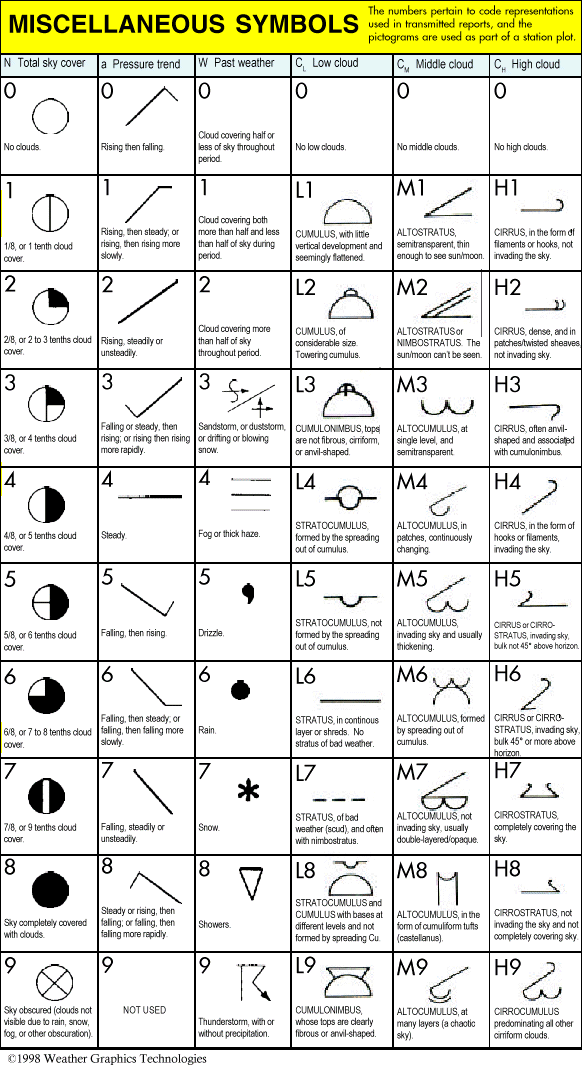
\includegraphics[width=0.6\textwidth]{Figs/wxcode2.png}
\caption{Example of standard graphical codification for cloud cover, pressure trend, past weather, and cloud types in a SYNOP report. Source: Weather Graphics Technologies.}\label{fig_synop_symbols_1}
\end{center}
\end{figure}

\begin{figure}[h]
\begin{center}
\includegraphics[width=0.4\textwidth]{Figs/partc_3.png}
\caption{Conventional codification for wind speed in a SYNOP report. Source: RMetS, The Royal Meteorological Society.}\label{fig_synop_symbols_2}
\end{center}
\end{figure}

\begin{figure}[h]
\begin{center}
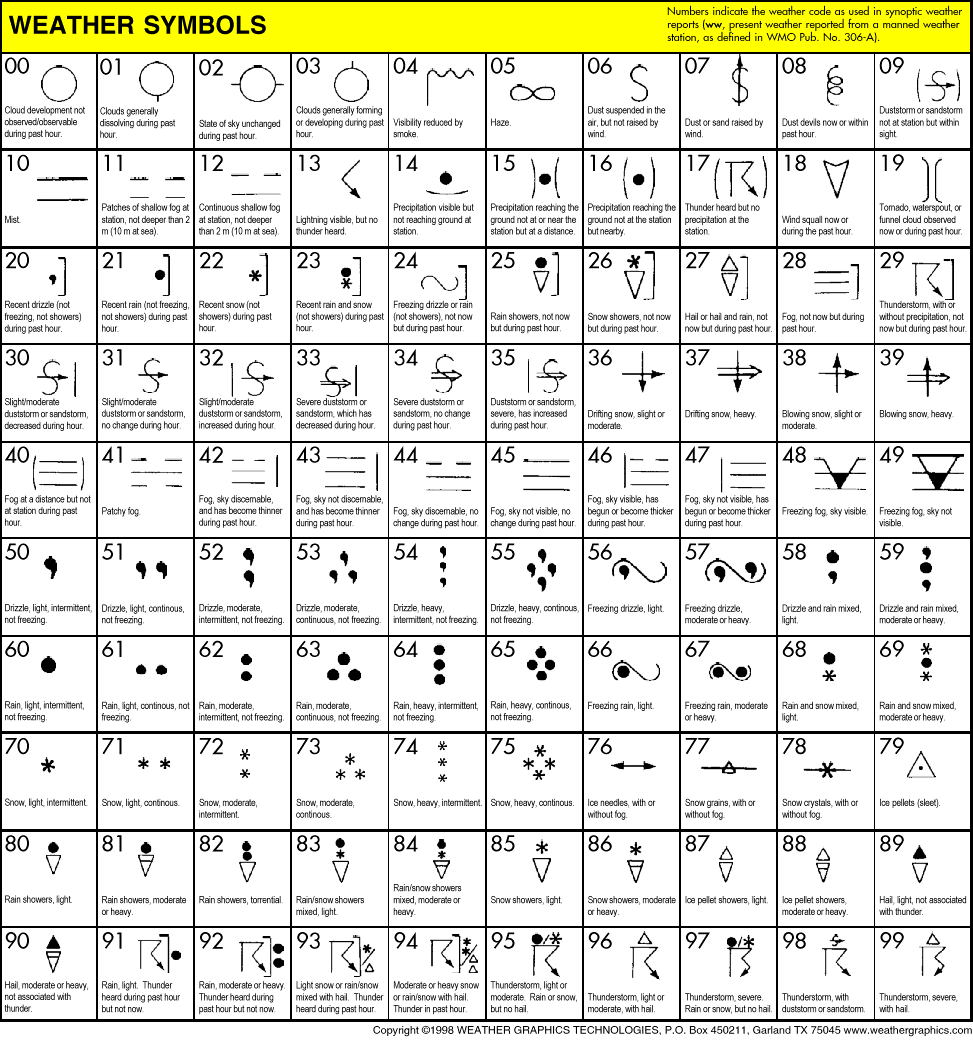
\includegraphics[width=0.8\textwidth]{Figs/wxcode1.png}
\caption{Example of standard graphical codification for present weather in a SYNOP report. Source: Weather Graphics Technologies.}\label{fig_synop_symbols_3}
\end{center}
\end{figure}


\newpage
\section{Results and Conclusions}


\nocite{WinNT}

%----------------------------------------------------------------------------------------

\bibliographystyle{abbrv}
%\bibliographystyle{apalike}

\bibliography{sample}

%----------------------------------------------------------------------------------------


\end{document}